\chapter{Related Work}
\label{cha:related-work}


\section{Graph Theory Basics}
\label{sec:graph-theory-basics}

In this section some graph theory related notation is defined, which is used during this thesis.
It is for the most part based on~\cite{Thulasiraman1992} and~\cite{Diestel2012}.

A graph is a mathematical construct that can be used to model and explore the relationship between objects.
More formally, a graph is a ordered pair of finite sets \( G = (V, E) \), whereas \( V \) denotes the set of \emph{vertices} (i.e., the objects) and \( E \subseteq [V]^{2} \) the set of \emph{edges} (i.e., the relationships between the objects).
It is common to write \( V(G) \) and \( E(G) \) to refer to the set of vertices and the set of edges respectively, that are associated with a graph \( G \).

An edge \( \{v_1, v_2\} \in E(G) \) is an unordered pair of two vertices.
Therefore, there is no distinction between the two edges \( \{v_1, v_2 \} \) and \( \{v_2, v_1\} \).
A graph with this property is called \emph{undirected}.
However, it is also possible to define edges as ordered pairs, such that each edge has a defined start and endpoint.
Such a graph is called \emph{directed}.

An edge of the form \( \{v_i, v_i\} \in E(G) \) is called a \emph{self-loop} of the vertex \( v_i \).
Furthermore, it is possible that two distinct vertices are joined by multiple edges.
Such edges are referred to as \emph{parallel} edges.
A graph that has no parallel edges and no self-loops is called \emph{simple}.
\Cref{fig:example_graphs} depicts an example for a simple graph and for a graph with parallel edges and a self-loop vertex.

It is also possible to assign each edge in a graph a real number, that adds additional information to it~\cite{Cormen2009}.
This number is usually called \emph{weight} and is determined by the function \( w : E(G) \rightarrow \mathbb{R} \).
This type of graph is called \emph{weighted} graph.
However, all further mentions and definitions for graphs are referring to undirected simple graphs unless stated otherwise.

It is possible to perform operations on graphs.
For instance, the union of two graphs \( G_{1} = (V_{1}, E_{1}) \) and \( G_{2} = (V_{2}, E_{2}) \) results in a graph \( G = (V_{1} \cup V_{2}, E_{1} \cup E_{2}) \).
Other binary operations, such as the intersection of two graphs, can be done analogously.
Unary operations on graphs are possible as well (e.g., the removal of vertices or edges).


\begin{figure}[h]
   \centering
   \begin{subfigure}[t]{0.45\textwidth}
     \centering
     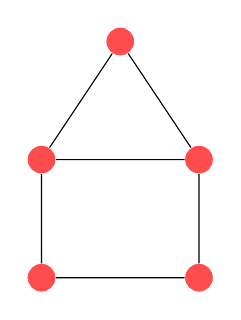
\begin{tikzpicture}[node/.style={circle,fill=red!70,minimum size=1em,inner sep=3pt]}]
       \node[node] (1) at (0, 0) {};
       \node[node] (2) at (-1, -1.5)  {};
       \node[node] (3) at (1, -1.5) {};
       \node[node] (4) at (-1, -3) {};
       \node[node] (5) at (1, -3) {};

       \draw (1) -- (3);
       \draw (1) -- (2) -- (4) -- (5) -- (3) -- (2);
     \end{tikzpicture}
     \caption{An undirected simple graph.}
   \end{subfigure}
   ~
   \begin{subfigure}[t]{0.45\textwidth}
     \centering
     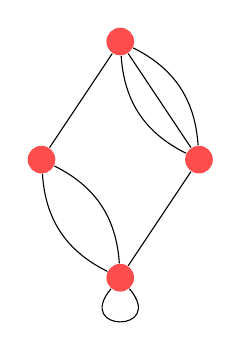
\begin{tikzpicture}[every loop/.style={}, node/.style={circle,fill=red!70,minimum size=1em,inner sep=3pt]}]
       \node[node] (1) at (0, 0) {};
       \node[node] (2) at (-1, -1.5)  {};
       \node[node] (3) at (1, -1.5) {};
       \node[node] (4) at (0, -3) {};

       \draw (1) -- (2);
       \draw (1) -- (3) -- (4);
       \path (2) edge [bend left] (4);
       \path (2) edge [bend right] (4);
       \path (3) edge [bend left] (1);
       \path (3) edge [bend right] (1);
       \draw (4) edge [in=-50,out=-130,loop] (4);
     \end{tikzpicture}
     \caption{An undirected graph with a self-loop and parallel edges.}
   \end{subfigure}

   \caption[Examples for graphs]{Graphical representation of two graphs with different properties.
   The vertices are represented by red dots and the edges are the line segments connecting them.}
\label{fig:example_graphs}
\end{figure}


The \emph{order} of a graph is the number of its vertices (i.e., the cardinality of the vertex set) and is denoted as \( n = |V(G)| \), whereas the cardinality of the edge set is usually denoted as \( m = |E(G)| \).
The neighborhood of a vertex \( v_i \) is defined as \( N(v_i) = \{v_j \in V(G) : \{v_i, v_j \} \in E(G)\} \).
It is the set of vertices that are adjacent to the vertex \( v_i \).
The cardinality of this set is called the \emph{degree} of the vertex and is denoted as \( d(v_i) = |N(v_i)| \).
A vertex without any neighbors (i.e., with a degree of zero) is called isolated.

It is often very useful to measure degree properties for a graph.
For example, the minimum degree \( \delta(G) = \min\{d(v_i) : v_i \in V(G)\} \), the maximal degree \( \Delta(G) = \max\{d(v_i) : v_i \in V(G)\} \), or the average degree \( d(G) = \frac{1}{n} \sum_{v_i \in V(G)} d(v_i) \).
An alternative way for the calculation of the average degree is \( d(G) = \frac{2m}{n} \).
This works since each edge is counted twice in the summation of the vertex degrees in the original formula.
These global measures can be used to gain insight into a graph's basic structure.

Another global property related to the degree is the degree distribution \( p \)~\cite{Barabasi2016} of a graph.
It yields the probability that a randomly selected vertex has a degree of \(k\).
Since it is a probability distribution \( \sum_{k=0}^\infty p(k) = 1 \) must hold.
The degree distribution for a given graph can be calculated by \( p(k) = \frac{|\{v \in V(G) \,:\, d(v) = k\}|}{n} \) for all possible values for \( k \) (i.e., by calculating the normalized degree histogram).

A \emph{path} on a graph can be defined as a finite sequence of vertices \( v_1,v_2,\dots,v_k \), such that between any consecutive pair of vertices exists an edge.
Furthermore, all edges between the vertices and the vertices itself must be distinct.
The first and the last vertices in the sequence are called the end vertices or terminal vertices of the path.

The \emph{path length} is the number of edges on the path.
Two vertices are \emph{connected} if it is possible to find a path with these two vertices as end points.
A vertex is, by definition, connected to itself.
If there exists a path between all pairs of vertices, then the graph is called connected.
It is always possible to partition the vertex and edge set of a disconnected graph in such a way, that there are no edges between vertices in different partitions.
These partitions are called the \emph{components} of the graph.

The \emph{clustering coefficient} of a vertex is a measure for the cliquishness of its neighborhood, and was introduced by \citet{Watts1998}.
A \emph{clique} in a graph is a subset of vertices, such that there exists an edge between every pair of vertices in this set.
The clustering coefficient \( C(v_i) \) is defined as the fraction of all possible edges between the neighbors of the vertex \( v_i \).
There exists at most \( \binom{d(v_i)}{2} = \frac{d(v_i)(d(v_i) - 1)}{2} \) edges between the vertices in the neighborhood.
Therefore, the clustering coefficient can be calculated by

\begin{equation}
 C(v_i) = \frac{2 \, |\{\{v_j, v_k\} \in E(G) : v_j \in N(v_i) \wedge v_k \in N(v_i)\}| }{d(v_i)(d(v_i) - 1)}.
\end{equation}

This is, of course, a local property of one vertex and is therefore sometimes called \emph{local clustering coefficient}.
However, it is also often useful to consider the average clustering coefficient \( C = \frac{1}{n} \sum_{v(i) \in V(G)} C(v_i) \) of the graph.
\Cref{fig:clustering-coefficient-examples} shows some examples for neighborhoods with local different clustering coefficients.
There is another definition of a \emph{global clustering coefficient}, which is also often called \emph{transitivity}~\cite{Boccaletti2006}.
It is defined as ratio of triangles (i.e., cliques consisting of exactly three vertices) to the number connected triples in the graph, i.e.,

\begin{equation}
 T = \frac{3 \times \text{\# of triangles}}{\text{\# of connected triples of vertices}}.
\end{equation}


\begin{figure}[h]
   \centering
   \begin{subfigure}[t]{0.31\textwidth}
     \centering
     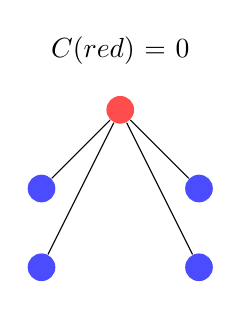
\begin{tikzpicture}[node/.style={circle,fill=red!70,minimum size=1em,inner sep=3pt]}, neighbor/.style={circle,fill=blue!70,minimum size=1em,inner sep=3pt]}]
       \node[text width=6em, align=center] at (0, 0.75)  {\(C(red) = 0\)};
       \node[node] (1) at (0, 0) {};
       \node[neighbor] (2) at (-1, -1)  {};
       \node[neighbor] (3) at (1, -1) {};
       \node[neighbor] (4) at (-1, -2)  {};
       \node[neighbor] (5) at (1, -2) {};

       \foreach \p in {2,3,4,5}{\draw (\p) -- (1); }
     \end{tikzpicture}
     \caption{In this example none of the four neighbors shares an edge with any other neighbor of the red vertex.
     Therefore, the clustering coefficient of the red vertex is \( \frac{0}{6} = 0 \).}
   \end{subfigure}
   ~
   \begin{subfigure}[t]{0.31\textwidth}
     \centering
     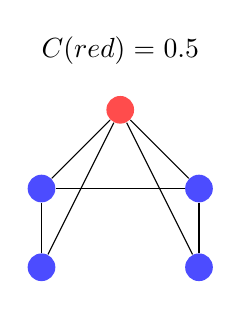
\begin{tikzpicture}[node/.style={circle,fill=red!70,minimum size=1em,inner sep=3pt]}, neighbor/.style={circle,fill=blue!70,minimum size=1em,inner sep=3pt]}]
       \node[text width=6em, align=center] at (0, 0.75)  {\(C(red) = 0.5\)};
       \node[node] (1) at (0, 0) {};
       \node[neighbor] (2) at (-1, -1)  {};
       \node[neighbor] (3) at (1, -1) {};
       \node[neighbor] (4) at (-1, -2)  {};
       \node[neighbor] (5) at (1, -2) {};

       \foreach \p in {2,3,4,5}{\draw (\p) -- (1); }
       \draw (2) -- (4);
       \draw (3) -- (5);
       \draw (3) -- (2);
     \end{tikzpicture}
     \caption{In this case, half of the possible edges between the neighbors are present.
     The clustering coefficient of the red vertex is \( \frac{3}{6} = \frac{1}{2} \).}
   \end{subfigure}
   ~
   \begin{subfigure}[t]{0.31\textwidth}
     \centering
     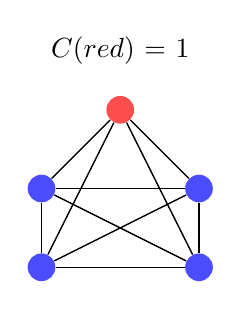
\begin{tikzpicture}[node/.style={circle,fill=red!70,minimum size=1em,inner sep=3pt]}, neighbor/.style={circle,fill=blue!70,minimum size=1em,inner sep=3pt]}]
       \node[text width=6em, align=center] at (0, 0.75)  {\(C(red) = 1\)};
       \node[node] (1) at (0, 0) {};
       \node[neighbor] (2) at (-1, -1)  {};
       \node[neighbor] (3) at (1, -1) {};
       \node[neighbor] (4) at (-1, -2)  {};
       \node[neighbor] (5) at (1, -2) {};

       \foreach \p in {1,2,3,4,5}{ \foreach \q in {1,2,3,4,5}{\draw (\p) -- (\q); }}
     \end{tikzpicture}
     \caption{The neighbors of the red vertex form a clique.
     Hence, the clustering coefficient of the red vertex is \( \frac{6}{6} = 1 \).}
   \end{subfigure}

   \caption[Clustering coefficient examples]{Examples for the local clustering coefficient of a vertex with a small neighborhood.
   The blue vertices are the neighbors of the red vertex.
   The possible number of edges between the four neighbors is \( \binom{4}{2} = 6 \).}
\label{fig:clustering-coefficient-examples}
\end{figure}


A connected triple is made up of three vertices as well, but does only have two edges between them.
Hence, a triangle consists of exactly three triples.
The global clustering coefficient is a measure for the extent of transitive connections in a graph (i.e., if there is an edge between vertices A and B, and between B and C, how likely is it that there is also an edge between A and C).
The two global clustering measures are, however, not equivalent to each other and may yield very different values~\cite{Newman2010} for the same graph.
The definition of the local clustering clustering coefficient introduces a bias towards vertices with smaller degree, due to smaller values in the denominator.
Therefore, the value for the average local clustering coefficient is possibly larger than the global clustering coefficient for the same graph, if the number of low-degree vertices is sufficiently large.


%% ========================================================================
%% ========================================================================


\section{Social Networks}
\label{sec:social-networks}

It is a common practice to use graphs to model the complex systems that arise in the real world.
For example, the web can be represented as a graph, where vertices correspond to websites and edges to the hyperlinks that connect them.
However, when modeling these large networks, it is common to use a terminology that is slightly different than the one used in the mathematical field of graph theory~\cite{Barabasi2016}.
In the context of networks vertices and edges are usually called \emph{nodes} and \emph{links} respectively.

Social networks~\cite{Newman2010} are another type of network that can benefit from the usage of graph theory methods.
The study of these networks is considered to be a part of the field of sociology and researchers may also use slightly different terminology for the vertices and edges in their work.
Nodes (or vertices) often represent people in social networks and are sometimes referred to as \emph{actors}.
However, it is also possible that they depict other entities, such as a departments, companies, or countries (i.e., larger groups of people).
The links (or edges) between these entities can denote, depending of the context, different things as well, and are sometimes referred to as \emph{ties}.
For example, links between persons can show social relationships (e.g., friendships), collaborations in projects (e.g., co-authorship of scientific papers), or other social interactions.
Links between companies could represent trading relationships or the like.

Social networks are often only mentioned in relation with large online communities, such as Facebook or Twitter, but there is no necessity that a social network must exist in an online form.
For instance, the network of acquaintances or friends in a school is considered a social network as well.
\Cref{fig:karate-club-network} shows a famous example of a small real-world social network.


\myfig{karate_club_network}
      {width=0.6\textwidth,height=0.6\textheight}
      {Zachary's karate club network~\cite{Zachary1977} is a social network that shows the relationship between 34 members of a university-based karate club in the US in the early 1970's.
      There exists an edge between two members if there were social interactions outside of the normal club activities between them (i.e., two members are considered friends).
      The graph shows a separation into two communities (red and blue nodes). This was caused by a dispute between the members of the club that was focused around two key persons.}
      {Zachary's karate club network}
      {fig:karate-club-network}


Two fundamental terms in the field of social network analysis are \emph{dyads} and \emph{triads}~\cite{Wasserman1994}.
These two concepts describe the relationship between multiple actors.
Dyads denote the linkage between pairs of actors and are used to study  pairwise relationships in social networks.
A triad on the other hand describes triples of actors and the ties between them.
This concept is especially important for the question of transitivity of certain relationships.
For instance, \enquote{is the friend of my friend also my friend?}.
The transitivity of trust, especially in the context of cryptography, is an interesting issue as well~\cite{Christianson1997}.

Another important concept is the strength of ties, which was introduced by \citet{Granovetter1973}.
The strength of a tie is influenced by factors like the time that two actors spend together, or the intimacy between them.
Depending on the strength, a tie can either be strong, weak, or absent.
Absent does not only include non-existing ties, but also ties with a strength that is below a certain threshold.
This concept of strong and weak ties can be used to explain the formation of triads.
If there already exists a strong tie between the two actors A and B, and between B and C, then there exists at least a weak tie between A and C.
This is true, due to the opportunities for the formation of a tie between A and C, that will result from a common strong tie to the actor B.
Furthermore, the spreading of information in social networks can be explained more accurately by taking the strength of ties into account.
Weak ties can help the flow of information by acting as bridges between sparsely connected parts of the network.

A property that many real-world social networks share are \emph{community structures}~\cite{Girvan2002}.
Communities are groups of actors that are more connected to actors in the same group, than to actors in different ones.
This basically means that in networks with community structures exist subsets of densely linked nodes and very few link links between the subsets.
The network shown in \cref{fig:karate-club-network} has two known communities highlighted by different node colors in the graph.

The detection of community structures in networks is a important research topic, since the identified communities may correspond to actual social groupings.
For example, the detected communities in a social network that models the friendship between students may represent the real corresponding social groups (i.e., the circles of friends).
There is a variety of different methods and approaches to perform this task.
Examples are algorithms based on hierarchical clustering, or edge betweenness (i.e., the number of shortest paths going through an edge)~\cite{Fortunato2010}.

However, it is often not feasible to study the network and its structure on a full global scale, due to processing limitations.
One alternative way is to consider single actors and their immediate neighborhood instead.
These small sub-networks are called \emph{egocentric} or \emph{personal} networks~\cite{Newman2010}.
Usually some number of these egocentric networks is sampled from the entire network and is examined for their local properties, such as the degree distribution or the local clustering coefficients.

Another attribute that many social networks share is that they are \emph{scale-free networks}~\cite{Barabasi2016}.
Formally, a network is a scale-free network if its degree distribution is a power-law (i.e., \( p(k) \sim k^{-\gamma} \), where \( \gamma \) is the parameter of the distribution that denotes the degree exponent).
The value for \( \gamma \) for most real-world (social) networks is in the range between 2 and 3.
A consequence of the power-law is that the distribution of the degrees is right-skewed and long-tailed.
This means that there is a large number of nodes in the network that have only a few links (i.e., a small degree) but there is also the chance that there exists a few nodes with a very high degree.
Such nodes are usually called \emph{hubs} and may correspond in the context of social networks to very influential actors that can play an important role in the network.

A property that social networks often show as well is the presence of the small-world effect.
The characteristic of small-world networks~\cite{Watts1999} is that even if the network is very large and sparsely connected, the average shortest path between any pair of nodes in it is usually very small.
For example, the famous experiment by \citet{Milgram1969} showed that it is possible to send a letter to a target by a chain of about six people on average, where each person in the chain is only allowed to forward the letter to acquaintances.
However, even tough there are some issues with the experimental setup of this study (e.g., a sample selection biases, or the sample size~\cite{Schnettler2009}), there is additional work in this area that supports the original findings.
For example, \citet{Leskovec2008} study of an online social network with 180 million nodes and 1.3 billion edges showed that the average path length in this network is 6.6, which is only slightly larger than in the original work.
Nonetheless, they showed that there exits paths up to a length of 29 as well.
A network with the small-world characteristic does usually exhibit two important properties.
First, the average shortest path length is small and only grows logarithmically with the size of the network, and second, it is highly clustered.
Note that the small-world effect does not only occur in social networks but also in many other real-world networks as well.
Examples are the US power grid network or the collaboration network of actors in movies~\cite{Watts1998}.


%% ========================================================================
%% ========================================================================


\section{Time-varying Networks}
\label{sec:time-varying-networks}

This section contains an overview on the concept of time-varying networks~\cite{Holme2012, Holme2015}.
Since this type of network is used in many different scientific fields it also has a variety of names.
For example, temporal networks, dynamic networks, evolving graphs, or the name that is mainly used in this thesis, time-varying networks.

As already mentioned in the section about social networks, the structure, or topology, of networks can be used to understand dynamic processes and their underlying behavior.
However, there are many dynamical processes that are modeled using static networks in which links are not active all the time.
One example would be a communication network, such as the network of phone calls between users.
Another example would be a social or collaboration network, where actors do not interact constantly but in irregular intervals.
These link activations at certain times can be very important to explain the dynamic process and are simply lost when approximated by a static graph.

The idea of time-varying networks is to introduce another dimension (i.e., time) to the network and move the information of when something happens from the dynamic process to the network itself.
As a general rule, a time-varying network is applicable when the structure (i.e., the topology) of the system and the temporal process are connected to each other.
This means that the time scale on which the network itself evolves should be similar to the time scale of the dynamic process that takes place on it.
For example, a time-varying network is not a suitable model for the internet, since the infrastructure (i.e., the topology) changes very slowly in comparison to the transmission of the packages that are routed through the network (i.e., the dynamic process).

The underlying concept of time-varying networks is called \emph{contacts} and can be seen as interactions between two nodes at a certain time.
The duration of the interaction is negligible and thus assumed to be instantaneous.
This is true at least in context of this thesis, however it is also possible to include the duration of interactions if necessary.
Contacts can be interpreted as an extension of links in static networks.
The unordered pair \( \{v_{i}, v_{j}\} \) becomes an ordered triple \( (v_{i}, v_{j}, t) \).
The order is in this case important, since the third object in the triple must refer to the time of interaction \(t\) between the nodes \( v_{i} \) and \( v_{j} \).

The usage of static networks in models for dynamic processes, which represent some time-dependent sequences of contacts between pairs of nodes, often results in a loss of information.
This sacrificed accurateness can possibly be avoided by using time-varying networks instead.
However, these temporal networks also introduce more complexity to the model, and one have to weight the gain in information versus the extra modeling effort.
For example, the case in which the information on how often something between two actors happened is way more important than when exactly it did, is a strong indicator for the preferred application of weighted graphs over their temporal counterpart (see \cref{fig:weighted-network-example} for an illustration of a weighted graph).

However, a simple graph without weights can also be used to approximate the interaction sequence of a time-varying network~\cite{Holme2013}.
The idea is to calculate a total weight for each pair of nodes in the network.
If the weight exceeds a certain threshold \( \Omega \in \mathbb{R}_{0}^{+} \) then there will be an edge between the two nodes in the static approximation.
Each contact between the pair in the sequence of contacts \( C \) contributes to the total weight.
However, contributions to the total decay exponentially with time.
Hence, the total weight \( w_{i,j} \) between two nodes \( v_{i} \) and \( v_{j} \) is \( w_{i,j} = \sum_{(v_{i}, v_{j}, t) \in C} \exp(\sfrac{-t}{\tau}) \), where \( \tau \) is an additional parameter that controls the exponential decay.
For a static approximation, that should contain an edge if there was at least one contact between the two nodes, can the threshold be set to \( \Omega = 0 \).
Networks that are generated using this approach are called exponential-threshold networks.

There are many different possibilities to represent a temporal network without the loss of information as well.
The simplest way to to this is by using the actual contact sequences.
A contact sequence is basically a list that contains all the contact triples.
This is a very raw form data (i.e., in essence a spreadsheet with three columns) and is therefore very easy to parse, and to use in algorithms.
However, the sequence is not very well suited for the analysis of the underlying dynamic process by humans, due to the lack of illustrations.

Another way to represent time-varying networks are graph sequences.
The idea behind them is to generate a static graph that contains all contacts between nodes in a given time window.
This method has the advantage that all tools that work for static graphs can also be applied to each of the graphs in the sequence.
The problem with this representation is, that the time resolution should be selected carefully to avoid the creation of graphs with no, or only a few, edges for most time steps.
\Cref{fig:graph-sequence-example} depicts an example of a graph sequence for a time-varying network with four nodes.

There exists more visual-focused representation methods as well.
One example would be the assignment of the series of contacts timestamps between two nodes to the corresponding link in the static network (see \cref{fig:time-stamp-edges-example} for an example).
This allows the usage of the variety of graph layout algorithms to visualize the network, but does not work very well for large networks due to the lack of space for the timestamps on the links and the large numbers of nodes.

A different idea for the visualization of a time-varying networks are contact timelines.
The interactions between nodes (i.e., the tuple of nodes that are interacting with each other) are placed on one axis and the time is placed on the other one.
A marker is set for each pair that interacts with each other at a certain time.
This allows for the visual detection of interaction patterns.
However, similar to the last representation method, this one is only reasonable for small networks as well.
\Cref{fig:timeline-example} shows an example for this type of representation.


\begin{figure}
   \centering
   \begin{subfigure}[t]{0.39\textwidth}
     \centering
     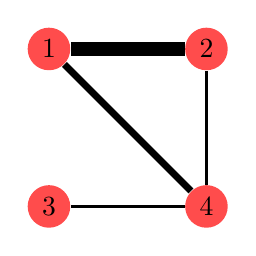
\begin{tikzpicture}[node/.style={circle,fill=red!70,minimum size=1em,inner sep=0pt,align=center,text width=14pt]}]

       \node[node] (1) at (0, 2) {1};
       \node[node] (2) at (2, 2) {2};
       \node[node] (3) at (0, 0) {3};
       \node[node] (4) at (2, 0) {4};

       \draw[line width=5.00pt] (1) -- (2);
       \draw[line width=2.50pt] (1) -- (4);
       \draw[line width=1.25pt] (2) -- (4);
       \draw[line width=1.25pt] (3) -- (4);
     \end{tikzpicture}

   \caption{Static approximation of the contact sequence as a weighted graph.
   The width of the lines between the nodes represents the weight (i.e., the total number of interactions between pairs of nodes).}
   \label{fig:weighted-network-example}
   \end{subfigure}
   ~
   \begin{subfigure}[t]{0.58\textwidth}
     \centering
     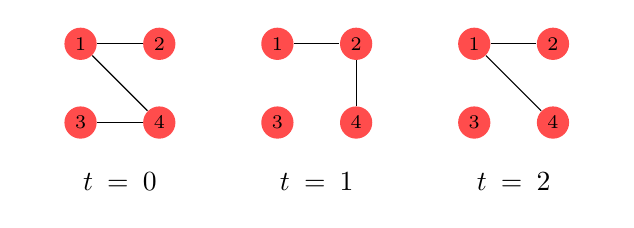
\begin{tikzpicture}[node/.style={circle,fill=red!70,minimum size=1em,inner sep=2pt]}]

       \foreach \t in {0, 1, 2} {
           \node[text width=6em, align=center] at (0.5+\t*2.5, -0.75)  {\(t=\t\)};
           \node[node] (1_\t) at (0+\t*2.5, 1) {\scriptsize 1};
           \node[node] (2_\t) at (1+\t*2.5, 1) {\scriptsize 2};
           \node[node] (3_\t) at (0+\t*2.5, 0) {\scriptsize 3};
           \node[node] (4_\t) at (1+\t*2.5, 0) {\scriptsize 4};
       }

       \draw (1_0) -- (2_0);
       \draw (1_0) -- (4_0);
       \draw (3_0) -- (4_0);
       \draw (2_1) -- (4_1);
       \draw (1_1) -- (2_1);
       \draw (1_2) -- (2_2);
       \draw (1_2) -- (4_2);
     \end{tikzpicture}

   \caption{Visualization of the graph sequence representation of the three time steps of a time-varying network.
   There exists an edge at the graph at time \( t \), if there was a contact between the two nodes at this time step.}
   \label{fig:graph-sequence-example}
   \end{subfigure}

   \begin{subfigure}[t]{0.39\textwidth}
     \centering
     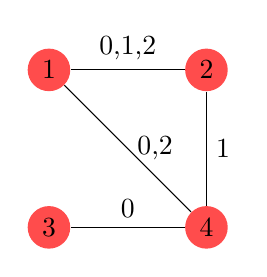
\begin{tikzpicture}[node/.style={circle,fill=red!70,minimum size=1em,inner sep=0pt,align=center,text width=14pt]}]

       \node[node] (1) at (0, 2) {1};
       \node[node] (2) at (2, 2) {2};
       \node[node] (3) at (0, 0) {3};
       \node[node] (4) at (2, 0) {4};

       \draw (1) -- (2) node[midway, above] {0,1,2};
       \draw (1) -- (4) node[midway, right] {0,2};
       \draw (2) -- (4) node[midway, right] {1};
       \draw (3) -- (4) node[midway, above] {0};
     \end{tikzpicture}

   \caption{A graph that contains an edge between two nodes if there was at least one contact between them.
   Furthermore, the edges are annotated with a time series of time steps that indicate when the interactions took place.}
   \label{fig:time-stamp-edges-example}
   \end{subfigure}
   ~
   \begin{subfigure}[t]{0.58\textwidth}
     \centering
     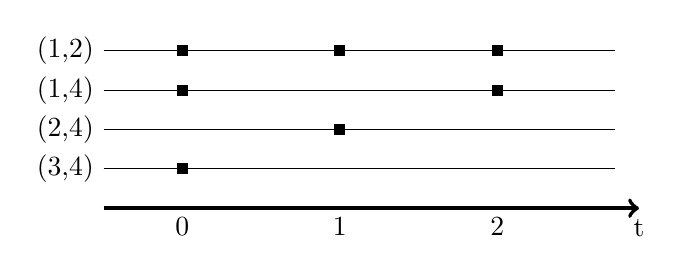
\begin{tikzpicture}[contact/.style={rectangle,fill=black,inner sep=0pt,minimum size=4pt]}]

       \draw (0, 2) node[left] {(1,2)} to (6.5, 2);
       \draw (0, 1.5) node[left] {(1,4)} to (6.5, 1.5);
       \draw (0, 1) node[left] {(2,4)} to (6.5, 1);
       \draw (0, 0.5) node[left] {(3,4)} to (6.5, 0.5);

       \draw[->, line width=1.5pt] (0, 0) to (6.8, 0) node[below] {t};
       \node[below] at (1, 0) {0};
       \node[below] at (3, 0) {1};
       \node[below] at (5, 0) {2};

       \node[contact] at (1, 2) {};
       \node[contact] at (1, 1.5) {};
       \node[contact] at (1, 0.5) {};
       \node[contact] at (3, 2) {};
       \node[contact] at (3, 1) {};
       \node[contact] at (5, 2) {};
       \node[contact] at (5, 1.5) {};
     \end{tikzpicture}

   \caption{Visualization of the contact sequence as a timeline of contacts.
   The vertical axis shows the interactions that happened between the nodes in the network and the horizontal axis shows the three time steps.
   There is a marker (depicted as a black rectangle) if there was a contact between the pair at a given time \( t \).}
   \label{fig:timeline-example}
   \end{subfigure}

   \caption[Graphical representations of time-varying networks]{(\subref{fig:graph-sequence-example})--(\subref{fig:timeline-example}) shows different representations for the contact sequence \( C = (1, 2, 0), (1, 4, 0), (3, 4, 0), (1, 2, 1), (2, 4, 1), (1, 2, 2), (1, 4, 2) \). (\subref{fig:weighted-network-example}) shows a static network of the same contact sequence, where the number of contacts between two nodes is reflected by the edge weights.}
\end{figure}


It is also noteworthy that most of the introduced measures for networks do not apply for temporal networks.
They must be redefined or extended.
For example, the concept of degree distributions does not exists in the context of time-varying networks.
But there are new measures like the \emph{inter-contact time distributions}, which describes the frequency of the time between contacts between either a specific pair or any two nodes.
Paths cannot be used in temporal networks as well, and are replaced by measures like \emph{latency} (i.e., how long since the last contact between two nodes) or \emph{temporal distance} (i.e., how long does it take to get from one node to another while taking the contacts into account).
There is also the idea, and many approaches, to extend community detection mechanisms for the usage in time-varying networks by running community detection algorithms for a static approximation of a network at time \( t \) and then refine the result by including community information from previous time steps.


%% ========================================================================
%% ========================================================================


\section{Generative Network Models}
\label{sec:network-models}

This section contains descriptions of different generative network models, which can be used to build graphs with certain characteristics.
They are often a useful tool when studying real-world networks (e.g., social networks) to gain a deeper understanding on the processes that creates them.


\subsection{The Erdős-Rényi Model}
\label{subsec:erdos-reni-model}

The Erdős–Rényi (ER) model~\cite{Erdos1959, Newman2010} was in its first form described by the two famous mathematicians Paul Erdős and Alfréd Rényi in 1959.
The model generates a random graph with \( n \) nodes and \( m \) links by choosing one of the \( \binom{\binom{n}{2}}{m} \) possible graphs of this size with equal probability at random.
It is sometimes also denoted as the \( G(n, m) \) model.

The basic idea behind this model is that large and complex networks often seem random and can be examined by using random graphs and statistical methods~\cite{Barabasi2002}.
Therefore, this very simple, yet powerful, model can be utilized to explore effects that take place in real-world systems.

There is another very similar model, the \( G(n, p) \) model, in which the number of links is not fixed beforehand.
The link quantity is determined by \( p \), the probability of the presence of a link between any pair of nodes in the network.
Hence, the edges of a random network are determined by flipping a biased coin for each of the \( \binom{n}{2} \) possible edges.

The probability for an arbitrary network with exactly \( m \) links under the \( G(n, p) \) model is \( p^{m} (1-p)^{\binom{n}{2} - m} \).
Therefore, the probability that the model will generate a network with \( m \) links is \( \prob{m} = \binom{\binom{n}{2}}{m} p^{m} (1-p)^{\binom{n}{2} - m} \) (i.e., the probability of such a network times the number of possible networks).
This corresponds to the binomial distribution \( B(\binom{n}{2}, p) \).
Hence, the expected value for the number of links is

\begin{equation}
    \expval{m} = \sum_{m=0}^{\binom{n}{2}} m \prob{m} = \binom{n}{2} p.
\end{equation}

The expected value for the average degree \( c \) of a network generated with this model is deduced in \cref{eq:avg-degree-erdos-model}.
The probability that an arbitrary node has a degree of exactly \( k \) is given by \( p(k) = \binom{n-1}{k} p^{k} (1-p)^{n-1-k} \) (i.e., \( k \) of its possible \( n-1 \) links must exist and there are \( \binom{n-1}{k} \) possible combinations for the \( k \) links).
Therefore, the degree distribution of this model is a binomial distribution as well.
However, it is also possible to approximate the degree distribution with a Poisson distribution \( p(k) = \exp(-c) \frac{c^{k}}{k!} \) for large values of \( n \).

\begin{equation}
  c = \expval{d(G)} = \sum_{m=0}^{\binom{n}{2}} \frac{2m}{n} \prob{m} = \frac{2}{n} \sum_{m=0}^{\binom{n}{2}} m \prob{m} = \frac{2}{n} \binom{n}{2} p = (n-1) p
  \label{eq:avg-degree-erdos-model}
\end{equation}

A nice property of the Erdős–Rényi model is that it can be used to study the formation of giant components.
The giant component of a network is a component that contains a large fraction of the nodes.
Others have adopted this model to study dynamic processes on it.
For example, \citet{Wang2003} are using it to study the spreading of viruses in networks, and \citet{Crucitti2004} for their research on cascading failures.
Hence, even such a simple model can be applied to study phenomenons that are part of many real-world networks.
Furthermore, it can be used to replicate the small average shortest path length, which grows logarithmically with the size of the network, and can  also observed in many real-world networks.

However, there are quite a few problems with this model as well.
The degrees in real-world networks are usually not binomial (or Poisson) distributed, but follow a power-law distribution.
Other examples for shortcomings of the model are the inability to generate community structures and hubs.


\subsection{The Barabási-Albert Model}
\label{subsec:barabasi-albert-model}

One model that addresses the problem of missing power-law degree distributions is the Barabási-Albert (BA) model~\cite{Barabasi2002}.
The model is named after its creators Réka Albert and Albert-László Barabási.
It tries to emulate the dynamic process that is responsible for the creation of scale-free degree distributions and yields a the generated network as result.

One of the main differences to the ER model is that the size of the network is not fixed.
The model starts with an small number of nodes and adds new ones to the network over time.
A newly added node forms links with already existing nodes.
What nodes are selected depends on how important they are.
The more important a node is, the more likely it is that the new nodes form connections with it.
This process is called \emph{preferential attachment}.
It can, for example, be used to explain the evolution of the online encyclopedia Wikipedia~\cite{Caldarelli2006}.
\citet{Eisenberg2003} showed that preferential attachment is the mechanism behind the evolution of protein networks.
Furthermore, new websites on the World-Wide-Web follow the same pattern, by linking already popular website more often~\cite{Barabasi1999}.

More formally, the model starts with a small number \( m_{0} \) of nodes and the following two steps are executed in every iteration:

\begin{enumerate}
    \item add a new node to the network
    \item choose \( m \leq m_{0} \) already existing nodes at random proportional to their degree and form a link between them and the newly added node
\end{enumerate}

Therefore, the degree of a node is a measure of its popularity and an existing node \( v_{i} \) will be selected with a probability \( \Pi(v_{i}) = \sfrac{d(v_{i})}{\sum_{j} d(v_{j})} \).
The process yields a network that consists of \( m_{0} + t \) nodes and \( m t \) links after \( t \) time steps.

It can be shown using different methods (e.g., continuum theory, master equations, or numerical), that the node degrees follow a power-law distribution with a degree exponent of \( \gamma = 3 \).
Furthermore, asymptotically does \( \gamma \) not depend on \( m \), the number of links that are generated in each iteration.
The degree distribution is also (asymptotically) independent of the time, and therefore on the size of the network.
This property of the model reflects the fact that there exists real-world networks of different sizes with power-law degree distributions.

However, like the ER model, the BA model has its shortcomings as well.
For example, the average path length of generated networks does not comply with real-world networks.
Another property that cannot be reproduced by this model are the community structures and the with it associated high clustering coefficient that many real-world, and especially social, networks have~\cite{Reid2011}.

Another interesting question regarding the Barabási-Albert model is if both mechanisms, the network growth and the preferential attachment, are necessary to produce scale-free networks.
The result of numerical simulations and formal tests of the model with one of the two mechanisms missing shows that both are indeed required.
Missing preferential attachment results in exponentially distributed node degrees, and while the absence of the network growth mechanism leads to a power-law degree distribution in the beginning, a shift to a normal distribution occurs over time~\cite{Barabasi2002}.
This indicates that, in fact, both mechanisms are required to yield networks with the scale-free property.


\subsection{Watts-Strogatz Model}
\label{subsec:watts-strogatz-model}

The model proposed by \citet{Watts1998} is able to produce networks with the small-world property.
The goal of it is to be as simple as possible while being able to replicate the effect~\cite{Watts2004}.
This is done by starting with a ring lattice graph with \( n \) nodes.
In such a graph are the nodes arranged uniformly on a ring and are connected to their \( k \) nearest neighbors on it.
This very regular graph has a high average local clustering coefficient and a high average shortest distance between any pair of nodes that grows linearly with the size of the network.
Therefore, it does not have the properties of small-world networks yet.

However, a simple rewiring process can introduce the small-world effect by changing the endpoints of some randomly selected edges.
This rewiring process depends on the parameter \( p \in [0, 1] \), which determines the probability for an edge to be rewired.
Note that this parameter is also sometimes refereed to as \( \beta \), since the model is known as Watts' beta model as well.

The rewiring process itself is very simple.
Each edge is rewired with probability \( p \).
The new endpoint of an edge is selected uniformly at random, but self-loops and parallel edges cannot be introduced in the network.


\myfig{watts-model}
      {width=0.75\textwidth,height=0.6\textheight}
      {Depiction of networks generated with the Watts-Strogatz model with an increasing value for \( p \). The initial ring lattice network consists of \( n = 20 \) nodes each with degree \( k = 4 \). Note that to ensure that the generated network stays connected \( n \) and \( k \) should be selected in such a way that \( n \gg k \gg \ln(n) \gg 1 \), which is not the case for this toy example. Figure borrowed from~\cite{Watts1998}.}
      {Watts-Strogatz model example}
      {fig:watts-model}


A rewiring probability of \( p = 1 \) changes the endpoint of every edge and produces a random network with properties similar to a network generated with the Erdős-Rényi model.
It exhibits a small average shortest path length, but also a small average local clustering coefficient.

However, networks generated with values for the rewiring probability in the range \( 0 < p < 1 \) can show the small-world property.
The effect of the rewiring process on the average path length in the network is substantial.
It drops immediately to a low value even if only a few edges get rewired.
This essentially produces shortcuts in the network by connecting nodes that are usually far apart, which decreases the average distance between any two nodes dramatically while keeping the average local clustering high.
Therefore, the model is able generate networks with small-world properties.

Nevertheless, if values of \( p \) get too large the average local clustering coefficient decreases significantly and the generated network resembles more and more a random network.
\Cref{fig:watts-model} illustrates the transformation of the network for increasing values of the rewiring probability.


%% ========================================================================
%% ========================================================================


\section{User Activity Models}
\label{sec:user-activity-models}

The modeling of the activity of users in complex systems (e.g., in social networks) can be a challenging task.
Usually the specific activities, such as writing of e-mails, posts on  Facebook, or tweets, are not of particular interest.
More relevant is how these events or activities laid out in time and what the distribution of intervals between two consecutive events is (i.e., the inter-event time distribution).

More formally, the sequence of timestamps of events for user \( i \) is written as \(t_{i,0}, t_{i,1}, t_{i,2}, \ldots \) with \( t_{i,j} \in \mathbb{N}_0 \), which is ordered in the sense that if \( t_{i,l} \ge  t_{i,k} \) then \( l \ge k \) and vice versa.
The inter-event times for the user \( i \) are defined as \( \tau_{i,j} = t_{i,j} - t_{i,j-1} \), for \(j = 1, 2, \ldots \) and their distribution is denoted as \( \varphi_{i} \).

There are various models that try to capture the patterns of human activities based on different approaches and some are discussed in this section.


\subsection{Stochastic Models}
\label{subsec:stochastic-models}

One of the simplest methods to model user activity is by using a Poisson process to describe the inter-activity times~\cite{Barabasi2005, Vazquez2006, Masuda2016}.
This stochastic process is defined by the event rate \( \lambda \), which states how often a event should occur in a given time window.
Two important properties of the Poisson process are that the inter-activity times are exponentially distributed and independent of each other.
This leads to the effect that events take place in regular intervals (i.e., at the given rate) and that it is almost impossible to have long periods of time between to consecutive activities.

However, it has been shown, that human activity patterns (e.g., email communication) cannot be modeled very accurately by a Poisson process due to its assumptions~\cite{Barabasi2005}.
Most activities are executed in bursts, followed by longer periods of inactivity.
For example, a person may have a dedicated time in the day for answering emails.
This behavior can be much better explained by a power-law distribution of the inter-activity times, since its long tail allows for longer periods of inactivity.

There are, however, approaches that try to tackle this problem by using extensions of Poisson processes.
For example, \citet{Malmgren2008} use a mixture of homogeneous and non-homogeneous Poisson processes to model user e-mail activity more precisely.
The rate of a non-homogeneous Poisson process does depend on the time, whereas the rate of a homogeneous process is constant.

An approach that does not only generate power-law distributed inter-event times, but also captures other patterns of human behavior, such as periodic spikes (e.g., higher activity every 24 hours) or a bimodal distribution of inter-event times (e.g., phases of high activity that are separated by phases of rest) was proposed by \citet{Costa2015}.
Their Rest-Sleep-and-Comment (RSC) model is based on the idea that a user can be in one of multiple states.
In the active state, a user generates events with a certain probability at a given rate, which depends on how much time has passed since the last event.
The rest and sleep states are used to model the inactivity of a user.
The difference between the two states is that the rest state produces null-events (i.e., it only increments the time) at a certain rate, whereas the sleep state is used to increment the time only once, but by a larger extent.
An active user can become inactive (i.e., go to the rest state) or stay active.
A user in the rest state can either become active, stay inactive, or go to the sleep state.
The user cannot stay in the sleep state, only go into the rest state again.
The state transition probabilities are parameters of the model.
This model was the foundation for a classifier, that is able to detect whether an activity sequence was generated by a bot or by a human with very high accuracy.

Another possibility to model the user activity in social networks is by using coupled Hidden Markov Models (CHMMs)~\cite{Raghavan2013}.
The Markov model has two hidden states that describe the user activity (active or inactive) and yields inter-activity times with respect to the current state.
The CHMM model takes the social network influence of other users into account as well, by explicitly coupling the stochastic processes of groups of people.
This is done by letting the transition probabilities between the states of the HMM for a single user be dependent on the activity of other users, that are in the circle of friends of the user (i.e., neighbors in the social network).
If the activity of the neighbors exceeds a certain threshold the probability for a user to become active gets larger.
The evaluation of this approach shows that this model is able to learn the complex human activity patterns and allows for highly accurate predictions.


\subsection{Queuing Models}
\label{subsec:queuing-models}

One approach, which successfully generates human activity patterns that follow a power-law distribution, are queuing models~\cite{Vazquez2006}.
The idea behind them is to think of a user as a queue that is constantly filled with new tasks (e.g., answer a email, go shopping, do the dishes,\ldots).
Each task takes a certain amount of time to finish and is prioritized by the user on arrival.
Furthermore, the queue is usually bounded in size, since people typically can only keep track of a certain amount of tasks at a time.
At each time step the user selects the task with the highest priority from the queue and executes it.

It can be shown that the time it takes for a task to be handled (i.e., the waiting time) follows a power-law distribution.
There is evidence that the waiting-time distribution of the queuing model is responsible for the inter-activity time power-law distribution of a specific activity.
This can possibly be explained by the observation that people tend to group tasks in categories and reinserting them into the queue with a lower priority after they are done.
For example, a person does not keep track of every unanswered email in the queue, but has an \enquote{answer email} task that contains all emails that need to be replied-to.
Therefore, this may lead to the answering of multiple emails in a short period of time, followed by a longer period of no email correspondence, due to the presence of other tasks with higher priority.


\subsection{Time-varying Network Models}
\label{subsec:time-varying-network-models}

The prior discussed user activity models are designed to solely describe the activity profile of a single person, or require at least a separate stochastic process for each one.
However, there are models that allow the description of the activities for multiple people at once using time-varying networks.

The difference between models for temporal networks and static network models (as described in~\cref{sec:network-models}) is, that the latter are purely connectivity driven~\cite{Perra2012a}.
This means that they are designed to generate specific topological properties in the networks (e.g., the formation of community structures, or short average path lengths), but do not consider the dynamic processes, which are responsible for these structures.

One of the simplest methods to generate a time-varying network of user activity was proposed by \citet{Holme2013}.
The idea is to generate a static network and assign each link a (possibly empty) set of timestamps, that represents the contact sequence between the two nodes.
To archive this, the first step is to generate a static network using the configuration model~\cite{Newman2010}.
This model assigns a number, drawn from a probability distribution (e.g., a power-law distribution), to each node in the network.
This number represents the number of \enquote{half edges} of the node.
These \enquote{half edges} can be seen as dangling edges that will be connected at random to other \enquote{half edges} of different nodes.
Therefore, this number corresponds to the degree of the node.
Self-loops and parallel edges are avoided during the matching process to generate a simple static network.
Next, each link in network is assigned a time window at random, in which contacts are possible (i.e., the activity interval).
In the last step of this approach, a time series of events is generated by drawing inter-event times from a power-law distribution.
This time series is then split into parts and mapped onto the activity windows of the nodes, thus, generating the contact sequences.

A different approach by~\citet{Perra2012a} is based on the idea of \emph{activity potentials}.
Each node \( v_{i} \) in the network of size \( n \) is assigned a quantity called the activity potential \( x_{i} \), which denotes the probability that the node will be active in a time window \( \Delta t \).
The activity potential for a user in real-world network can be determined by calculating the ratio of the number of interactions of this user to the total number of interactions in a time window.
The measuring of the activity potentials for multiple users usually yields long-tailed distributions of the quantity, which corresponds to typical heterogeneous human activity patterns~\cite{Vazquez2006, Jo2012}.
Furthermore, the size of the time window, which is used to estimate the probabilities, seems not to effect the resulting distribution in a significant way.

The first step of this activity-driven model is to initialize each node in the network by assigning it a activity/firing rate \( a_{i} = \eta x_{i} \), where the activity potential is drawn from a suitable probability distribution \( f(x) \) and \( \eta \) is a rescaling factor that is chosen in such a way that the expected number of active nodes in the time window is \( \eta \expval{x} n \).
The range of possible activity potential values is \( x_{i}\ \in [\varepsilon, 1] \).
This lower bound \( \varepsilon \) of the activity potential is necessary to avoid possible divergences of the distribution for values that are very close to zero~\cite{Clauset2009}.

The time-varying network can be generated after this short initial setup phase by repeating the following instructions for each time step \( t \):

\begin{enumerate}
    \item Create a new network \( G_{t} \), that contains all \( n \) nodes but has no links yet.
    \item Every node \( v_{i} \) becomes active with probability \( a_{i} \Delta t \). Active nodes choose \( m \) distinct other nodes uniformly at random and form links with them.
    \item Increment the current time \( t \rightarrow t + \Delta t \).
\end{enumerate}

Therefore, in this model the time-varying networks are represented as sequences of graphs (see \cref{sec:time-varying-networks}), which are called \emph{instantaneous networks} in the context of this model.

The cardinality of the edge set after time \( t \) is given by \( |E_{t}| = m \eta \expval{x} n \), since every active node creates exactly \( m \) links.
Therefore, the average degree of the instantaneous network at time \( t \) is

\begin{equation}
    d(G_{t}) = \frac{2|E_{t}|}{n} = \frac{2 m \eta \expval{x} n}{n} = 2 m \eta \expval{x}.
\end{equation}

The probability for a node to become active does not change over time and is, therefore, also independent of previous activities.
This resembles the problem already encountered with models based on Poisson processes.
The inter-event times for a node \(v_{i}\) will eventually be exponential distributed \(\varphi_{i}(\tau) = a_{i} \exp(-a_{i} \tau)\)~\cite{Moinet2016}.
Additionally, the model lacks of realism in the sense that every node selects its neighbors in each iteration uniformly at random, which leads to networks with a random structure.
Typically users are prone to repeat previous communication~\cite{Karsai2014}.

Nevertheless, this model possesses a few considerable advantages.
First, and most important, it produces not only activities for a single user, but generates snapshots of the total user activities in the network in each time window.
Furthermore, it is a very simple model.
It only requires a few parameters and the activity potential distribution governs the dynamical behavior in the network.

Moreover, this model can be used to explain the formation heterogeneous structures (i.e., hubs) in networks over longer periods of time.
This is done by examining the \emph{integrated network} \(G_{T} = \bigcup_{t=0}^{T} G_{t}\), which is defined as the union of all instantaneous networks up to the time stamp \(T\) (see \cref{fig:integrated-network-example} for an example).
It can be shown that the  degree distribution of this integrated network has the form \(p_{T}(k) \sim f(\frac{k}{T m \eta})\).
Therefore, it is up to a rescaling factor the same as the activity potential distribution.
Hence, the model is able to generate scale-free networks by drawing the activity potentials from a power-law distribution.
The resulting hubs are not caused by preferential attachment like in other models, but due to the heterogeneous activity profiles of the nodes.
The rescaling factor emerges from the fact that the model does not capture all features of real-world networks.
For instance, memory effects are not present that would allow links, which were formed in earlier instantaneous networks, to be formed later again with higher probability.


\begin{figure}
    \centering
    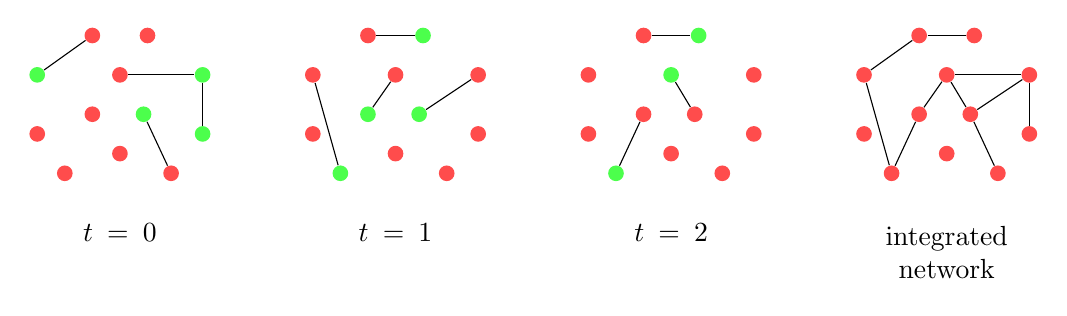
\begin{tikzpicture}[node/.style={circle,fill=red!70,minimum size=0.1em,inner sep=2pt]}, active/.style={circle,fill=green!70,minimum size=0.1em,inner sep=2pt]}]

        \node[text width=6em, align=center] at (1.05, -0.5)  {\(t=0\)};
        \node[active] (1) at (0, 1.5) {};
        \node[node]   (2) at (0.7, 2) {};
        \node[node]   (3) at (1.4, 2) {};
        \node[active] (4) at (2.1, 1.5) {};
        \node[node]   (5) at (1.05, 1.5) {};
        \node[node]   (6) at (0.7, 1) {};
        \node[active] (7) at (1.35, 1) {};
        \node[node]   (8) at (1.05, 0.5) {};
        \node[node]   (9) at (0.35, 0.25) {};
        \node[node]   (10) at (1.7, 0.25) {};
        \node[node]   (11) at (0, 0.75) {};
        \node[active] (12) at (2.1, 0.75) {};
        \draw (1) -- (2);
        \draw (4) -- (5);
        \draw (4) -- (12);
        \draw (7) -- (10);

        \node[text width=6em, align=center] at (1.05+1*3.5, -0.5)  {\(t=1\)};
        \node[node]   (1) at (0+1*3.5, 1.5) {};
        \node[node]   (2) at (0.7+1*3.5, 2) {};
        \node[active] (3) at (1.4+1*3.5, 2) {};
        \node[node]   (4) at (2.1+1*3.5, 1.5) {};
        \node[node]   (5) at (1.05+1*3.5, 1.5) {};
        \node[active] (6) at (0.7+1*3.5, 1) {};
        \node[active] (7) at (1.35+1*3.5, 1) {};
        \node[node]   (8) at (1.05+1*3.5, 0.5) {};
        \node[active] (9) at (0.35+1*3.5, 0.25) {};
        \node[node]   (10) at (1.7+1*3.5, 0.25) {};
        \node[node]   (11) at (0+1*3.5, 0.75) {};
        \node[node]   (12) at (2.1+1*3.5, 0.75) {};
        \draw (2) -- (3);
        \draw (5) -- (6);
        \draw (4) -- (7);
        \draw (9) -- (1);

        \node[text width=6em, align=center] at (1.05+2*3.5, -0.5)  {\(t=2\)};
        \node[node]   (1) at (0+2*3.5, 1.5) {};
        \node[node]   (2) at (0.7+2*3.5, 2) {};
        \node[active] (3) at (1.4+2*3.5, 2) {};
        \node[node]   (4) at (2.1+2*3.5, 1.5) {};
        \node[active] (5) at (1.05+2*3.5, 1.5) {};
        \node[node]   (6) at (0.7+2*3.5, 1) {};
        \node[node]   (7) at (1.35+2*3.5, 1) {};
        \node[node]   (8) at (1.05+2*3.5, 0.5) {};
        \node[active] (9) at (0.35+2*3.5, 0.25) {};
        \node[node]   (10) at (1.7+2*3.5, 0.25) {};
        \node[node]   (11) at (0+2*3.5, 0.75) {};
        \node[node]   (12) at (2.1+2*3.5, 0.75) {};
        \draw (5) -- (7);
        \draw (9) -- (6);
        \draw (2) -- (3);

        \node[text width=6em, align=center] at (1.05+3*3.5, -0.75)  {integrated network};
        \node[node] (1) at (0+3*3.5, 1.5) {};
        \node[node] (2) at (0.7+3*3.5, 2) {};
        \node[node]   (3) at (1.4+3*3.5, 2) {};
        \node[node] (4) at (2.1+3*3.5, 1.5) {};
        \node[node] (5) at (1.05+3*3.5, 1.5) {};
        \node[node]   (6) at (0.7+3*3.5, 1) {};
        \node[node]   (7) at (1.35+3*3.5, 1) {};
        \node[node]   (8) at (1.05+3*3.5, 0.5) {};
        \node[node]   (9) at (0.35+3*3.5, 0.25) {};
        \node[node]   (10) at (1.7+3*3.5, 0.25) {};
        \node[node]   (11) at (0+3*3.5, 0.75) {};
        \node[node] (12) at (2.1+3*3.5, 0.75) {};
        \draw (1) -- (2);
        \draw (4) -- (5);
        \draw (4) -- (12);
        \draw (2) -- (3);
        \draw (5) -- (6);
        \draw (4) -- (7);
        \draw (9) -- (1);
        \draw (5) -- (7);
        \draw (9) -- (6);
        \draw (7) -- (10);

    \end{tikzpicture}
    \caption[Integrated network example]{Illustration for the formation of the integrated network for a small example with \( n = 12 \) nodes. The first three graphs show the instantaneous networks for the time steps \( t = 0 \), \( t = 1 \), and \( t = 2 \). In each time step a few nodes get active (green nodes) and establish links to \( m = 1 \) other nodes. The forth graph shows the integrated network up to \( T = 2 \). It contains all links that were established in the instantaneous networks. Parallel links are not allowed (i.e. a link is only added once to the integrated network even if it is present in multiple time steps).}
    \label{fig:integrated-network-example}
\end{figure}


Regardless of its simplicity, this activity-driven model can help to understand topological patterns and the dynamics of systems (e.g., epidemic spreading processes).
\citet{Starnini2013}, for example, study the topological properties of this model in a more formal way by mapping it onto a hidden variables network model.
The idea behind hidden variables models is that the probability of the formation of a link between two nodes depends on some underlying characteristic of the nodes (i.e., the hidden variables).
In this case the hidden variable is the activity potential.
A network that was generated using this model fully depends on probability distributions that are related to the hidden variables.
Therefore, topological properties also depend on these probability distributions and can be expressed with respect to them.
The properties of the degree distribution of the integrated network could be verified using this more formal approach.
In addition, they showed that the clustering coefficient of the network is rather small and comparable to the clustering coefficient of random networks.
They also propose to use the hidden-variable approach to study possible extensions of the model, which is, for example, done for the NoPAD model~\cite{Moinet2015}, that is briefly discussed later in this section.

The activity-driven model is also a fundamental framework for many other studies that use it as start point for their work.
For example, \citet{Perra2012b} use this model to study random walks on temporal networks, or \citet{Rizzo2016} are applying it for their research on the spreading of the infectious Ebola disease in Liberia.
Another paper by \citet{Rizzo2014} uses the activity-driven network framework to study how an epidemic effects the behavior of persons.
They showed that a reduction of the activity potential of persons, due to the fact that they are already ill or because they are trying to protect them self from the disease, may help the slow down the spreading process.
A paper on a similar topic by \citet{Liu2014} proposes a framework to develop strategies on how to contain the spreading of diseases.
\citet{Mistry2015} use the model to explore the spreading of opinions in social networks.
They showed that activists are able to spread messages across the population more effectively and can help to reduce the cost of campaigns.

On the other hand, others try to improve the model by making it more realistic by introducing additional mechanisms.
\citet{Laurent2015} add additional social mechanisms (e.g., memory) to the model to allow for the formation of communities in the integrated network.
This model is explained in great detail in \cref{sec:underlying-model}, since it is used as a foundation for our work presented in this thesis.
Another extension by \citet{Moinet2015, Moinet2016} solves the problem of inaccurate inter-events times by making the activity potential of each node time dependent.
This model is known as the non-poissonian activity-driven (NoPAD) model and can generate inter-event time distributions that can also be observed in real-world networks.
\citet{Wang2016} proposed the Activity-Security-Trust (AST) model, which not only considers activity as the explicit driving force behind dynamic processes, but also incorporates the implicit factors security and trust.
Trust can be interpreted as the belief in honesty or fairness between two nodes and influences the possible link formation between them.
The second extension, the security level, is like the activity potential a property of each node that determines how well a node is prepared against possible attacks.
It can be seen as the probability of a node to accept the interaction initiated by another one.
\citet{Sunny2015} add link lifetimes to the activity-driven framework.
Every time a link is formed it is assigned a lifetime, that is drawn at random from a probability distribution.
This link may then be part of multiple consecutive instantaneous networks
and is only removed after its lifetime has decayed, in contrast to the simple activity-driven model, where links are meant to be instantaneous and are deleted after every time step.
The authors use this new introduced mechanism to study how well link lifetimes are suited to model disease spreading processes.
While \citet{Laurent2015} examine the local effects that are responsible for the formation of complex network structures using the activity-driven framework, takes \citet{Alessandretti2017} work also the global effects for the formation of links into account.
Each node in the model is not only assigned an activity potential, but also a attractiveness quantity, which determines how popular a node is in the network.
Nodes that are more popular get selected more often from active nodes.
This basically corresponds to an preferential attachment process.
They not only show in their work that activity and the attractiveness are correlated in real-world social and collaboration networks, but also that this influences dynamical processes on the network in a significant way.


%% ========================================================================
%% ========================================================================


\section{Peer Influence}
\label{sec:peer-influence}

Peer influence or peer pressure plays an important role in the field of sociology and psychology.
There are a lot of studies that investigate how peer influence affects the behavior of people in different settings.
This is not only done for for real-world social networks (e.g., a social network of students in a school), but also for online social and collaboration networks, such as Facebook or StackOverflow.

These studies often investigate peer effects for harmful behavior like smoking or drinking\footnote{\url{https://xkcd.com/1534/}}~\cite{Simons2001, Powell2005}.
\citet{Krasnova2008} showed that peer pressure is an important factor for adolescents to participate in online social networks, and \citet{Huang2014} concluded in their work that being exposed to pictures of drinking and smoking friends on social media websites may lead to an adaption of these behaviors.

However, peer influence is not necessarily a bad thing.
For example, \citet{Smith1984} showed that the introduction of peer monitors in a kindergarten classroom decreased non-participation and disruptive behavior of the other children.
Another example is the study conducted by \citet{Christakis2008}.
They examined a relatively large social network of approximately 12,000 people over more than 30 years and evaluated the spreading of smoking in the network.
The results of this study  not only showed that the number of smokers declined over the years, but also that clusters of smokers in the network seem to disappear at roughly the same time.
This indicates that people that quit smoking may trigger a cascading cessation effect in their social circle.
For instance, they showed that in their data set the smoking cessation of a spouse reduces the probability for the other one to smoke by 67\%.

Peer influence plays an important role in opinion dynamics models as well.
The formation and diffusion of opinions in complex networks is examined in these models.
Opinions can be trivial things like taste in food and entertainment, or more sophisticated issues like political views, and are usually heavily influenced by others~\cite{Acemoglu2011}.

One popular use case for these types of models are voter models, which try to maximize the number of voters for a political party in a election (i.e., the opinion) with a minimum amount of cost that is associated with winning voters over.
For instance, the voter model by \citet{Masuda2015} considers two different types of voters, the partisan voters (often also referred to as zealots), which do not change their opinion, and independent voters, which can.
An independent voter adapts a political view proportionally to the presence of this view in its neighborhood and with respect to zealots that influence him or her.
It can be used to determine the optimal set of nodes in the network of independent voters, that should be controlled and influenced by zealots of one party to obtain the maximum number of voters.

In another work by \citet{Estrada2013} is the effect of peer influence on reaching consensus in social groups examined.
They model the influence between two user as their social distance, which is a function of the length of the shortest path between them in the social network.
This allows for a node to receive indirect peer pressure from other nodes that are not directly connected to it (i.e., do not share an edge) as well.
They showed that this indirect peer influence is not only important for reaching consensus in social groups, but also for social group leaders to emerge, which affects the opinions in the entire network and helps to reduce the time until consensus is reached.

Another interesting application for the usage of peer influence are network models that incorporate peer effects on the activity of nodes.
For instance, \citet{Walk2016} proposed a model that helps to study how the activity in large collaboration and social networks develops over longer time spans and what effects the micro-behavior of users (i.e., their intrinsic activity and the influence on their neighbors) has on the macro-behavior of the system.
The macro-behavior of the system can be interpreted as the overall activity in the network.
This helps to understand how some systems can archive a state in which the can become self-sustaining, in the sense that no external influences or stimuli are needed to keep the network permanently active, while others become non-active very quickly, even after lots of activity in the early stages of the network.

Their model is based on the idea that each user has an intrinsic activity, which declines over time.
This can be interpreted as the growing loss of interest of users in the system.
But there is also an opposite force, the peer influence of others, that motivates the user to contribute.

More formally, the model is defined as a dynamic process that takes place on a network, were users are represented as nodes and there exists a link between two users if they interacted or collaborated at some point.
Furthermore, every user \( v_{i} \) is assigned a positive real-valued variable \( a_{i} \), which represents the activity of the user.
The dynamic process is then defined by the following system of coupled non-linear differential equations:

\begin{equation}
    \frac{\mathrm{d} a_{i}}{\mathrm{d} t} =  \underbrace{f(a_{i})}_{\text{activity decay}} + \underbrace{\sum_{j \in N(v_{i})} g(a_{j})}_{\text{peer influence}} \,\, \text{ for } i = 1,2,\ldots,n
\end{equation}

The first part of the right hand side of the equation represents the intrinsic activity decay of a user, and the function \( f \) defines how fast the loss of activity should occur.
In their work a linear function \( f(a_{i}) = -\lambda a_{i} \) is used, where \( \lambda > 0 \) denotes the rate on which the activity decays.
This leads to an exponential decay of the user activity.
The second part of the equation denotes the positive peer influence of the users neighbors.
This is based on the idea that active neighbors may also increase the activity of a user, due to a boost in their motivation to participate in the network.
The function \( g \) determines the level of positive peer influence of a neighbor, and is selected to be the algebraic sigmoid function \( g(a_{i}) = \sfrac{q a_{i}}{\sqrt{a_{c}^{2} a_{j}^{2}}} \).
This function introduces two additional parameter to the model, \( a_{c} > 0 \) controls what level of activity of a neighbor is required such that it influences a user in a significant way, and \( q > 0 \) determines the maximum amount of peer influence activity that a neighbor can transfer to another user.

In their work they perform a linear stability analysis on the system of differential equations and show that the stability of the system is determined by the relation between the activity dynamics ratio \( \frac{\lambda}{\mu} \) (with \( \mu = \frac{q}{a_{c}} \)) and the topological structure of the network.
This means to prevent the network from becoming or staying inactive, there must either be constant external influences to keep the activity up or the system needs to become unstable.
This can be done, for example, by changing the network structure (e.g., removing links) or by manipulating the three model parameter.

Furthermore, they apply their activity dynamics model to some real-world data sets.
For instance, different instances of StackExchange collaboration networks and various wikis.
This is done by first estimating the ratio \( \frac{\lambda}{\mu} \) from the activity in the data sets, and then simulating the activity in the networks.
However, due to some limitations and approximations in the parameter estimation is a highly accurate prediction of the activity not possible.
Nevertheless, the model is able to predict trends in the activity of a empirical network by simulating its activity dynamics quite well and, therefore, provide additional confidence in the validity of the model.

Additionally, two stability measures for social or collaboration networks are introduced in this work.
First, the system mass is defined as the inverse of the normalized standard deviation of the activity dynamics ratio, and indicates the robustness of a system with respect to change of the activity dynamics parameter.
The second measure is called activity momentum and is defined as product of the system mass and the over some time span averaged last observed activity in the network, and is an improved indicator for the robustness.
For instance, a system with a large activity momentum value handles the sudden inactivity of a considerable number of users better, since it can retain most of its activity.
Therefore, much more \enquote{force} is needed to render a network with high activity momentum inactive.

Another interesting question in the context of peer influence effects in networks was raised in the work of \citet{Aral2009}.
They suggested that the behavior of a user in a network may not be entirely driven by the influence of its peers, but can be explained in large parts by homophily.
Homophily (also known as assortativity or assortative mixing) is the effect that users tend to interact with other users that are similar to them self.
They examined a temporal network of instant-message communication between users and studied how the adaption of a new feature in the messaging application could be explained.
The idea behind their work is that users may not adapt the feature shortly after their friends because of peer influence, but do it simply because they behave similar to them anyway.
For instance, users that have the property of being early-adopters are more likely to be friends with early-adopters as well, and therefore, start using the feature at about the same time.
They proposed a statistical framework that is able to distinguish between peer influence and homophily, and showed that other methods overestimate the share of influenced adaption by a factor of four to eight, and that at least half of the adaption in their instant-messaging data set was introduced by homophily.
